\documentclass{CInf_practice}

\sheet{8}{Schaltwerke \& Register-Transfer-Ebene}
\usetikzlibrary{automata,positioning,arrows.meta} 

\begin{document}
\cinftitle

\ex{Füllstandsregelung}{4 + 6 + 12 + 8 = 30}

\subex{Ein- \& Ausgangssignale, Modulbild}
\noindent Eingaben:
\begin{enumerate}[align=left,leftmargin=\marginparwidth]
   \item[$X_t$] Sensor oben (top), 1 = feucht, 0 = trocken
   \item[$X_m$] Sensor mitte (middle), 1 = feucht, 0 = trocken
   \item[$X_b$] Sensor unten (bottom), 1 = feucht, 0 = trocken
\end{enumerate}
Ausgaben:
\begin{enumerate}[align=left,leftmargin=\marginparwidth]
   \item[$Y$] Abflusssteuerung, 1 = öffnen, 0 = schließen
   \item[$E$] Errorsignal, 1 = Error, 0 = kein Error
\end{enumerate}

\usetikzlibrary{shapes.misc}
\tikzset{bus/.style={strike out,
                     draw,
                     -,
                     append after command={
                        node[above=.5ex of \tikzlastnode] {\tiny #1}
                     }
                     }
        }
\begin{center}
  \begin{tikzpicture}
    % module
    \draw (2,3) rectangle node {Sicherheitsfüllstandregler (SFR)} +(6,-2);
    % in
    \draw[<-] (2,2.5) -- node[bus={1}] {} ++(-1,0) node[left] {$X_t$};
    \draw[<-] (2,2) -- node[bus={1}] {} ++(-1,0) node[left] {$X_m$};
    \draw[<-] (2,1.5) -- node[bus={1}] {} ++(-1,0) node[left] {$X_b$};
    % out
    \draw[->] (8,2) -- node[bus={1}] {} ++(1,0) node[right] {$Y$};
  \end{tikzpicture}
\end{center}


\subex{Zustandsgraph}

\begin{center}
  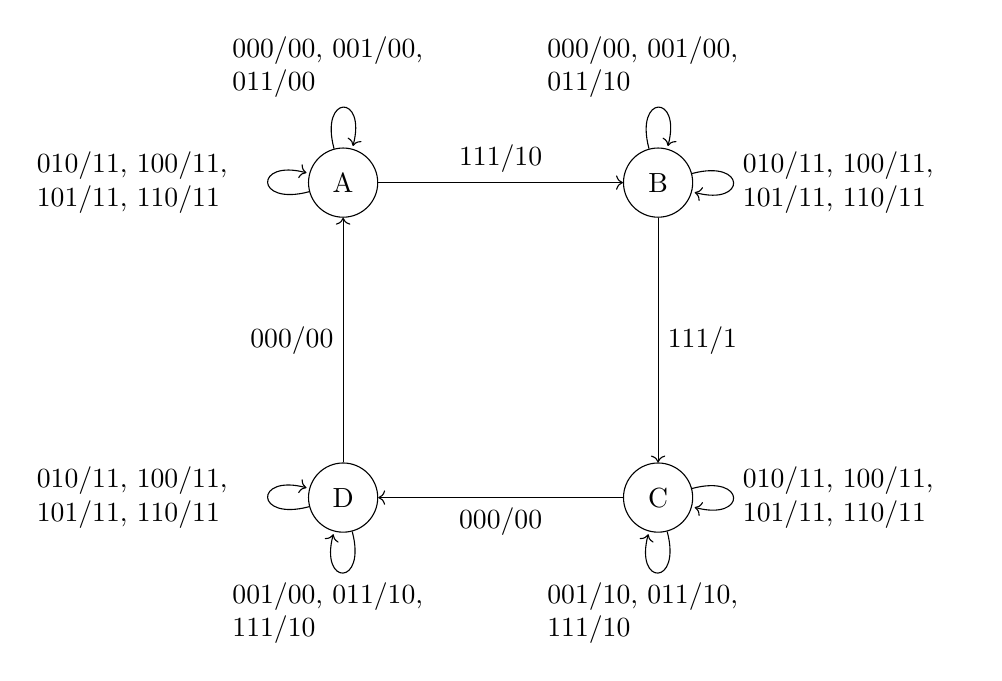
\begin{tikzpicture}[node distance=4cm]
    \node[state] (A) {A};
    \node[state,right of=A] (B) {B};
    \node[state,below of=B] (C) {C};
    \node[state,left of=C] (D) {D};
    
    \path[->] % inlet
              (A) edge[loop above] node[above, text width=8em] {000/00, 001/00, 011/00} (A) % valid
              (A) edge[loop left]  node[left, text width=8em]  {010/11, 100/11, 101/11, 110/11} (A) % error
              (A) edge             node[above]                 {111/10} (B) % next
  
              % hold it
              (B) edge[loop above] node[above, text width=8em] {000/00, 001/00, 011/10}(B) % valid
              (B) edge[loop right] node[right, text width=8em] {010/11, 100/11, 101/11, 110/11}(B) % error
              (B) edge             node[right]                 {111/1}(C) % next
              
              % outlet
              (C) edge[loop below] node[below, text width=8em] {001/10, 011/10, 111/10}(C) % valid
              (C) edge[loop right] node[right, text width=8em] {010/11, 100/11, 101/11, 110/11}(C) % error
              (C) edge             node[below]                 {000/00}(D) % next
              
              % hold it
              (D) edge[loop below] node[below, text width=8em] {001/00, 011/10, 111/10}(D) % valid
              (D) edge[loop left]  node[left, text width=8em]  {010/11, 100/11, 101/11, 110/11}(D) % error
              (D) edge             node[left]                  {000/00}(A) % next
              ;
              
  \end{tikzpicture}
\end{center}
\begin{center}
  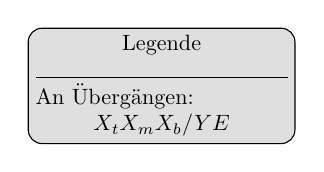
\begin{tikzpicture}
    \node[scale=.8,draw,rounded corners=5pt,fill=lightgray!50,text width=4cm] (legend) {
       \makebox[4cm]{Legende}\\
       \hrulefill \\
       %An Zuständen: \makebox[4cm]{$$} \\ 
       An Übergängen: \makebox[4cm]{ $X_tX_mX_b/YE$ }
    };
  \end{tikzpicture}
\end{center}

Der Graph ist konsistent und vollständig.


\subex{Zustandsübergangstabelle \& -codierung}
Vier Zustände erlauben eine Codierung mit $\log_2{4}=2$ Bits. Es scheint sinnvoll, zwischen zwei Zuständen die Hamming distance klein zu halten. Es ist möglich, Codierungen zu finden, bei der für jeden Zustandswechsel nur ein Bit geändert wird. Wir wählen deswegen:

\begin{ctabular}{c|m}
Zustand & $Codierung $ = Q_1Q_0 \\\hline
A & 00 \\
B & 10 \\
C & 11 \\
D & 01 \\
\end{ctabular}

Für die Realisierung mit JK-Flipflops wird das linke Bit durch das $JK_1$-FF, das recht durch das $JK_0$-FF kodiert. Dabei stehen in der Tabelle $JK_1^{n+1} = Q_1^{n+1}$ bzw. $JK_0^{n+1} = Q_0^{n+1}$ für die jeweiligen Ausgänge, d.h. $1 = Q$ und $0 = \comp Q$.

\begin{ctabular}{cc|mmm|mm|c|mmm|mmm}
$Z^n$ & $(Q_1Q_0)^n$ &  X_t & X_m & X_b & Y & E & $(Q_1Q_0)^{n+1}$
      & J_1^n & K_1^n & Q_1^{n+1} & J_0^n & K_0^n & Q_0^{n+1} \\ \hline % do the JK's make sense?
A & 00 & 0 & 0 & 0 & 0 & 0 & 00 & 0 & 1 & 0 & 0 & 1 & 0 \\
A & 00 & 0 & 0 & 1 & 0 & 0 & 00 & 0 & 1 & 0 & 0 & 1 & 0 \\
A & 00 & 0 & 1 & 0 & 1 & 1 & 00 & 0 & 1 & 0 & 0 & 1 & 0 \\
A & 00 & 0 & 1 & 1 & 0 & 0 & 00 & 0 & 1 & 0 & 0 & 1 & 0 \\
A & 00 & 1 & 0 & 0 & 1 & 1 & 00 & 0 & 1 & 0 & 0 & 1 & 0 \\
A & 00 & 1 & 0 & 1 & 1 & 1 & 00 & 0 & 1 & 0 & 0 & 1 & 0 \\
A & 00 & 1 & 1 & 0 & 1 & 1 & 00 & 0 & 1 & 0 & 0 & 1 & 0 \\
A & 00 & 1 & 1 & 1 & 1 & 0 & 01 & 0 & 0 & 0 & 1 & 0 & 1 \\ \hline
B & 01 & 0 & 0 & 0 & 0 & 0 & 01 & 0 & 0 & 0 & 1 & 0 & 1 \\
B & 01 & 0 & 0 & 1 & 0 & 0 & 01 & 0 & 0 & 0 & 1 & 0 & 1 \\
B & 01 & 0 & 1 & 0 & 1 & 1 & 01 & 0 & 0 & 0 & 1 & 0 & 1 \\
B & 01 & 0 & 1 & 1 & 0 & 0 & 01 & 0 & 0 & 0 & 1 & 0 & 1 \\
B & 01 & 1 & 0 & 0 & 1 & 1 & 01 & 0 & 0 & 0 & 1 & 0 & 1 \\
B & 01 & 1 & 0 & 1 & 1 & 1 & 01 & 0 & 0 & 0 & 1 & 0 & 1 \\
B & 01 & 1 & 1 & 0 & 1 & 1 & 01 & 0 & 0 & 0 & 1 & 0 & 1 \\
B & 01 & 1 & 1 & 1 & 1 & 0 & 11 & 1 & 0 & 1 & 1 & 0 & 1 \\ \hline
C & 11 & 0 & 0 & 0 & 0 & 0 & 10 & 1 & 0 & 1 & 0 & 1 & 0 \\
C & 11 & 0 & 0 & 1 & 1 & 0 & 11 & 1 & 0 & 1 & 1 & 0 & 1 \\
C & 11 & 0 & 1 & 0 & 0 & 1 & 11 & 1 & 0 & 1 & 1 & 0 & 1 \\
C & 11 & 0 & 1 & 1 & 1 & 0 & 11 & 1 & 0 & 1 & 1 & 0 & 1 \\
C & 11 & 1 & 0 & 0 & 0 & 1 & 11 & 1 & 0 & 1 & 1 & 0 & 1 \\
C & 11 & 1 & 0 & 1 & 0 & 1 & 11 & 1 & 0 & 1 & 1 & 0 & 1 \\
C & 11 & 1 & 1 & 0 & 0 & 1 & 11 & 1 & 0 & 1 & 1 & 0 & 1 \\
C & 11 & 1 & 1 & 1 & 1 & 0 & 11 & 1 & 0 & 1 & 1 & 0 & 1 \\ \hline
D & 10 & 0 & 0 & 0 & 0 & 0 & 00 & 0 & 1 & 0 & 0 & 1 & 0 \\
D & 10 & 0 & 0 & 1 & 0 & 0 & 10 & 1 & 0 & 1 & 0 & 1 & 0 \\
D & 10 & 0 & 1 & 0 & 1 & 1 & 10 & 1 & 0 & 1 & 0 & 1 & 0 \\
D & 10 & 0 & 1 & 1 & 0 & 0 & 10 & 1 & 0 & 1 & 0 & 1 & 0 \\
D & 10 & 1 & 0 & 0 & 1 & 1 & 10 & 1 & 0 & 1 & 0 & 1 & 0 \\
D & 10 & 1 & 0 & 1 & 1 & 1 & 10 & 1 & 0 & 1 & 0 & 1 & 0 \\
D & 10 & 1 & 1 & 0 & 1 & 1 & 10 & 1 & 0 & 1 & 0 & 1 & 0 \\
D & 10 & 1 & 1 & 1 & 1 & 0 & 10 & 1 & 0 & 1 & 0 & 1 & 0 \\ \hline
\end{ctabular}


\subex{Ansteuergleichungen}
Die Wertetabelle wurde zuvor ergänzt. Die Gleichungen können stark vereinfacht werden, da die Zustände nur in wenigen Sonderfällen wechseln. Das Ausnutzen der Hamming distance erlaubt es also im Grunde, die Ansteuergleichungen indirekt durch die vier Zustandswechsel zu definieren.

\begin{align*} % if needed we can simplify this further
Q_0^{n+1} = Q_0^{n} \comp{Q_1^n \comp{X_t} \comp{X_m} \comp{X_b}} + \comp{Q_1^n}\, \comp{Q_1^n} X_t X_m X_b \\
Q_1^{n+1} = Q_1^{n} \comp{Q_0^n \comp{X_t} \comp{X_m} \comp{X_b}} + \comp{Q_1^n}\,       Q_0^n  X_t X_m X_b
\end{align*}



\ex{Konverter}{6 + 12 + 6 + 6 = 30}
\subex{Flowdiagram}
\begin{center}
  \begin{tikzpicture}
    \node[cloud] (Begin) {begin};
    \node[decision, below left=of Begin] (VALID) {VALID=1?};
    \node[block, below=of VALID.south,text width=10em] (store)
          {NUM[0] \la INBUS(0:3)\\NUM[1] \la INBUS(4:7)\\NUM[2] \la INBUS(8:11)};
    \node[block, below=of store,text width=14em] (convout0)
          {READY \la 1\\OUTBUS \la NUM[0] + $0110000_2$};
    \node[block, right=of convout0,text width=14em] (convout1)
          {READY \la 1\\OUTBUS \la NUM[1] + $0110000_2$};
    \node[block, above=of convout1,text width=14em] (convout2)
          {READY \la 1\\OUTBUS \la NUM[2] + $0110000_2$};
    \draw[line] (Begin) -| (VALID);
    \draw[line] (VALID) -- node[left]{yes} (store);
    \draw[line] (store) -- (convout0);
    \draw[line] (convout0) -- (convout1);
    \draw[line] (convout1) -- (convout2);
    \draw[line] (convout2) |- (Begin);
    \draw[line] (VALID) -| node[below, near start] {no} (Begin.south);
  \end{tikzpicture}
\end{center}


\subex{RTeasy Programm}
{
  \lstset{xleftmargin=0pt,xrightmargin=0pt}
  \lstinputlisting{8.2_Konverter.rt}
}


\subex{Zustände, Kontrollsignale und Kriterien}

Die Zustände, Kontrollsignale und Kriterien sind im Code markiert.

\bigskip

\textbf{Zustände:}

\begin{itemize}
	\item \texttt{WAITLOAD}: Wartet auf \texttt{VALID=1} und lädt bei Erfolg.
  \item \texttt{OUTx}: geben jeweils \texttt{NUM[x]} aus.
\end{itemize}

Die Anzahl Zustände kann durch eine Zählvariable auf zwei reduziert werden.

\bigskip

\textbf{Kontrollsignale:}

Ein Kontrollsignal ist \texttt{goto BEGIN}. Wir bezeichnen es mit \emph{back}. Hinzu kommt das Kontrollsignal, \texttt{READY} zu setzen. Wir nennen es \texttt{setReady}. 

\bigskip

\textbf{Kriterien:}

Das einzige Kriterium ist \texttt{VALID=1}. Wir bezeichnen es im Blockschaltbild mit \emph{load}.


\subex{Blockschaltbild}
% it's easy to see that I have no clue what they expect us to do here...
\begin{center}
  \begin{tikzpicture}
    \draw (1.5,8) rectangle node{READY} ++(3,1);
    \draw (5.5,8) rectangle node{VALID} ++(3,1);
    
    \draw (2.5,6) rectangle node{INBUS} ++(5,1);
    
    \draw (0,3) rectangle node{NUM[0]} ++(3,1);
    \draw (3.5,3) rectangle node{NUM[1]} ++(3,1);
    \draw (7,3) rectangle node{NUM[2]} ++(3,1);
    
    \draw (2.5,0) rectangle node{OUTBUS} ++(5,1);
    
    % load
    \draw[-] (7,8) -- node{/} node[left] {1} ++(0,-1);
    \draw[-o] (8.5,8.5) -- ++(.5,0) node[right] {\emph{load}};
    
    \draw[->] (2.75,6) -- node{/} node[left] {4} ++(0,-2);
    \draw[->] (5,6) -- node{/} node[left] {4} ++(0,-2);
    \draw[->] (7.25,6) -- node{/} node[left] {4} ++(0,-2);

    % write
    \draw[->] (2.75,3) -- node{/} node[left] {7} ++(0,-2);
    \draw[->] (5,3) -- node{/} node[left] {7} ++(0,-2);
    \draw[->] (7.25,3) -- node{/} node[left] {7} ++(0,-2);
    
    % do we need these six?
    \draw[o-] (2.75,4.5) --  ++(-.5,0) node[left]{\emph{in}};
    \draw[o-] (5,4.5) --  ++(-.5,0) node[left]{\emph{in}};
    \draw[o-] (7.25,4.5) --  ++(-.5,0) node[left]{\emph{in}};
    
    \draw[o-] (2.75,1.5) --  ++(-.5,0) node[left]{\emph{out0}};
    \draw[o-] (5,1.5) --  ++(-.5,0) node[left]{\emph{out1}};
    \draw[o-] (7.25,1.5) --  ++(-.5,0) node[left]{\emph{out2}};

    % setReady
    \draw[o-] (1.5,8.5) -- ++(-.5,0) node[left] {\emph{setReady}};
   
    % Steuerwerk
    \draw (13,0) rectangle node[rotate=-90] {Steuerwerk} ++(1,9);
    \draw[o-] (13,7.5) -- ++(-.5,0) node[left] {\emph{load}};
    \draw[-o] (13,6.5) -- ++(-.5,0) node[left] {\emph{setReady}};
    \draw[-o] (13,5.5) -- ++(-.5,0) node[left] {\emph{in}};
    \draw[-o] (13,3.5) -- ++(-.5,0) node[left] {\emph{out0}};
    \draw[-o] (13,2.5) -- ++(-.5,0) node[left] {\emph{out1}};
    \draw[-o] (13,1.5) -- ++(-.5,0) node[left] {\emph{out2}};
  \end{tikzpicture}
\end{center}


\ex{Minimumsuche in RTeasy}{4 + 10 + 11 + 7 + 3 + 5 = 40}
\subex{Blockschaltbild}


\subex{Flowchart}

\begin{center}
   \begin{tikzpicture}
      \node[cloud] (begin) {Begin};
      \node[block,below=of begin] (clrar) {AR \la 0 \\ MinAdr \la 0};
      \node[block,below=of clrar] (lddr) {DR \la Memory[AR]};
      \node[block,below=of lddr] (ldmin) {Min \la DR};
      \node[decision,below=of ldmin] (areq31) {AReq31=1};
      \node[block,below=of areq31] (incrar) {AR \la AR + 1};
      \node[block,below=of incrar] (lddr2) {DR \la Memory[AR]};
      \node[block,below=of lddr2] (lda) {A \la DR};
      \node[decision,below=of lda] (minbiga) {Minbiga=1};
      \node[block,below=of minbiga] (ldminadr) {MinAdr \la AR};

      \node[block,left=of areq31] (ldar) {AR \la MinAdr};
      \node[block,below=of ldar] (lddr3) {DR \la Mem[AR]};
      \node[block,below=of lddr3] (ldout) {OUTBUS \la DR};
      \node[cloud,below=of ldout] (end) {End};

      \draw[->] (begin) -- (clrar);
      \draw[->] (clrar) -- (lddr);
      \draw[->] (lddr) -- (ldmin);
      \draw[->] (ldmin) -- (areq31);
      \draw[->] (areq31) -- node[right] {No} (incrar);
      \draw[->] (incrar) -- (lddr2);
      \draw[->] (lddr2) -- (lda);
      \draw[->] (lda) -- (minbiga);
      \draw[->] (minbiga) -- node[right] {Yes} (ldminadr);
      \draw[->] (minbiga.east) -- ++(2cm,0) node[above,pos=.3] {No}  coordinate (c) |- (areq31.east);
      \draw     (ldminadr.east) -| (c);
      \draw[->] (areq31.west) -- node[above] {Yes} (ldar);
      \draw[->] (ldar) -- (lddr3);
      \draw[->] (lddr3) -- (ldout);
      \draw[->] (ldout) -- (end);
   \end{tikzpicture}
\end{center}

\subex{RTeasy Programm}


\subex{Kriterien und Signale}

\begin{center}
   \begin{tabularx}{.8\textwidth}{|L|X|}
      \hline
      \normalfont{\textbf{Kriterien}} & \textbf{Funktion} \\ \hline
      MinbigA   & 1, wenn $Min > A$ \\
      AReq31    & 1, wenn $AR=31$ \\ \hline
      \hline
      \normalfont{\textbf{Kontrollsignale}} & \textbf{Funktion} \\ \hline
                                            & \\
   \end{tabularx}
\end{center}


\subex{Taktzahl}


\subex{Technische Realisierung}



\end{document}
